\section{Welcome Screens}

\begin{figure}[H]
    \centering
    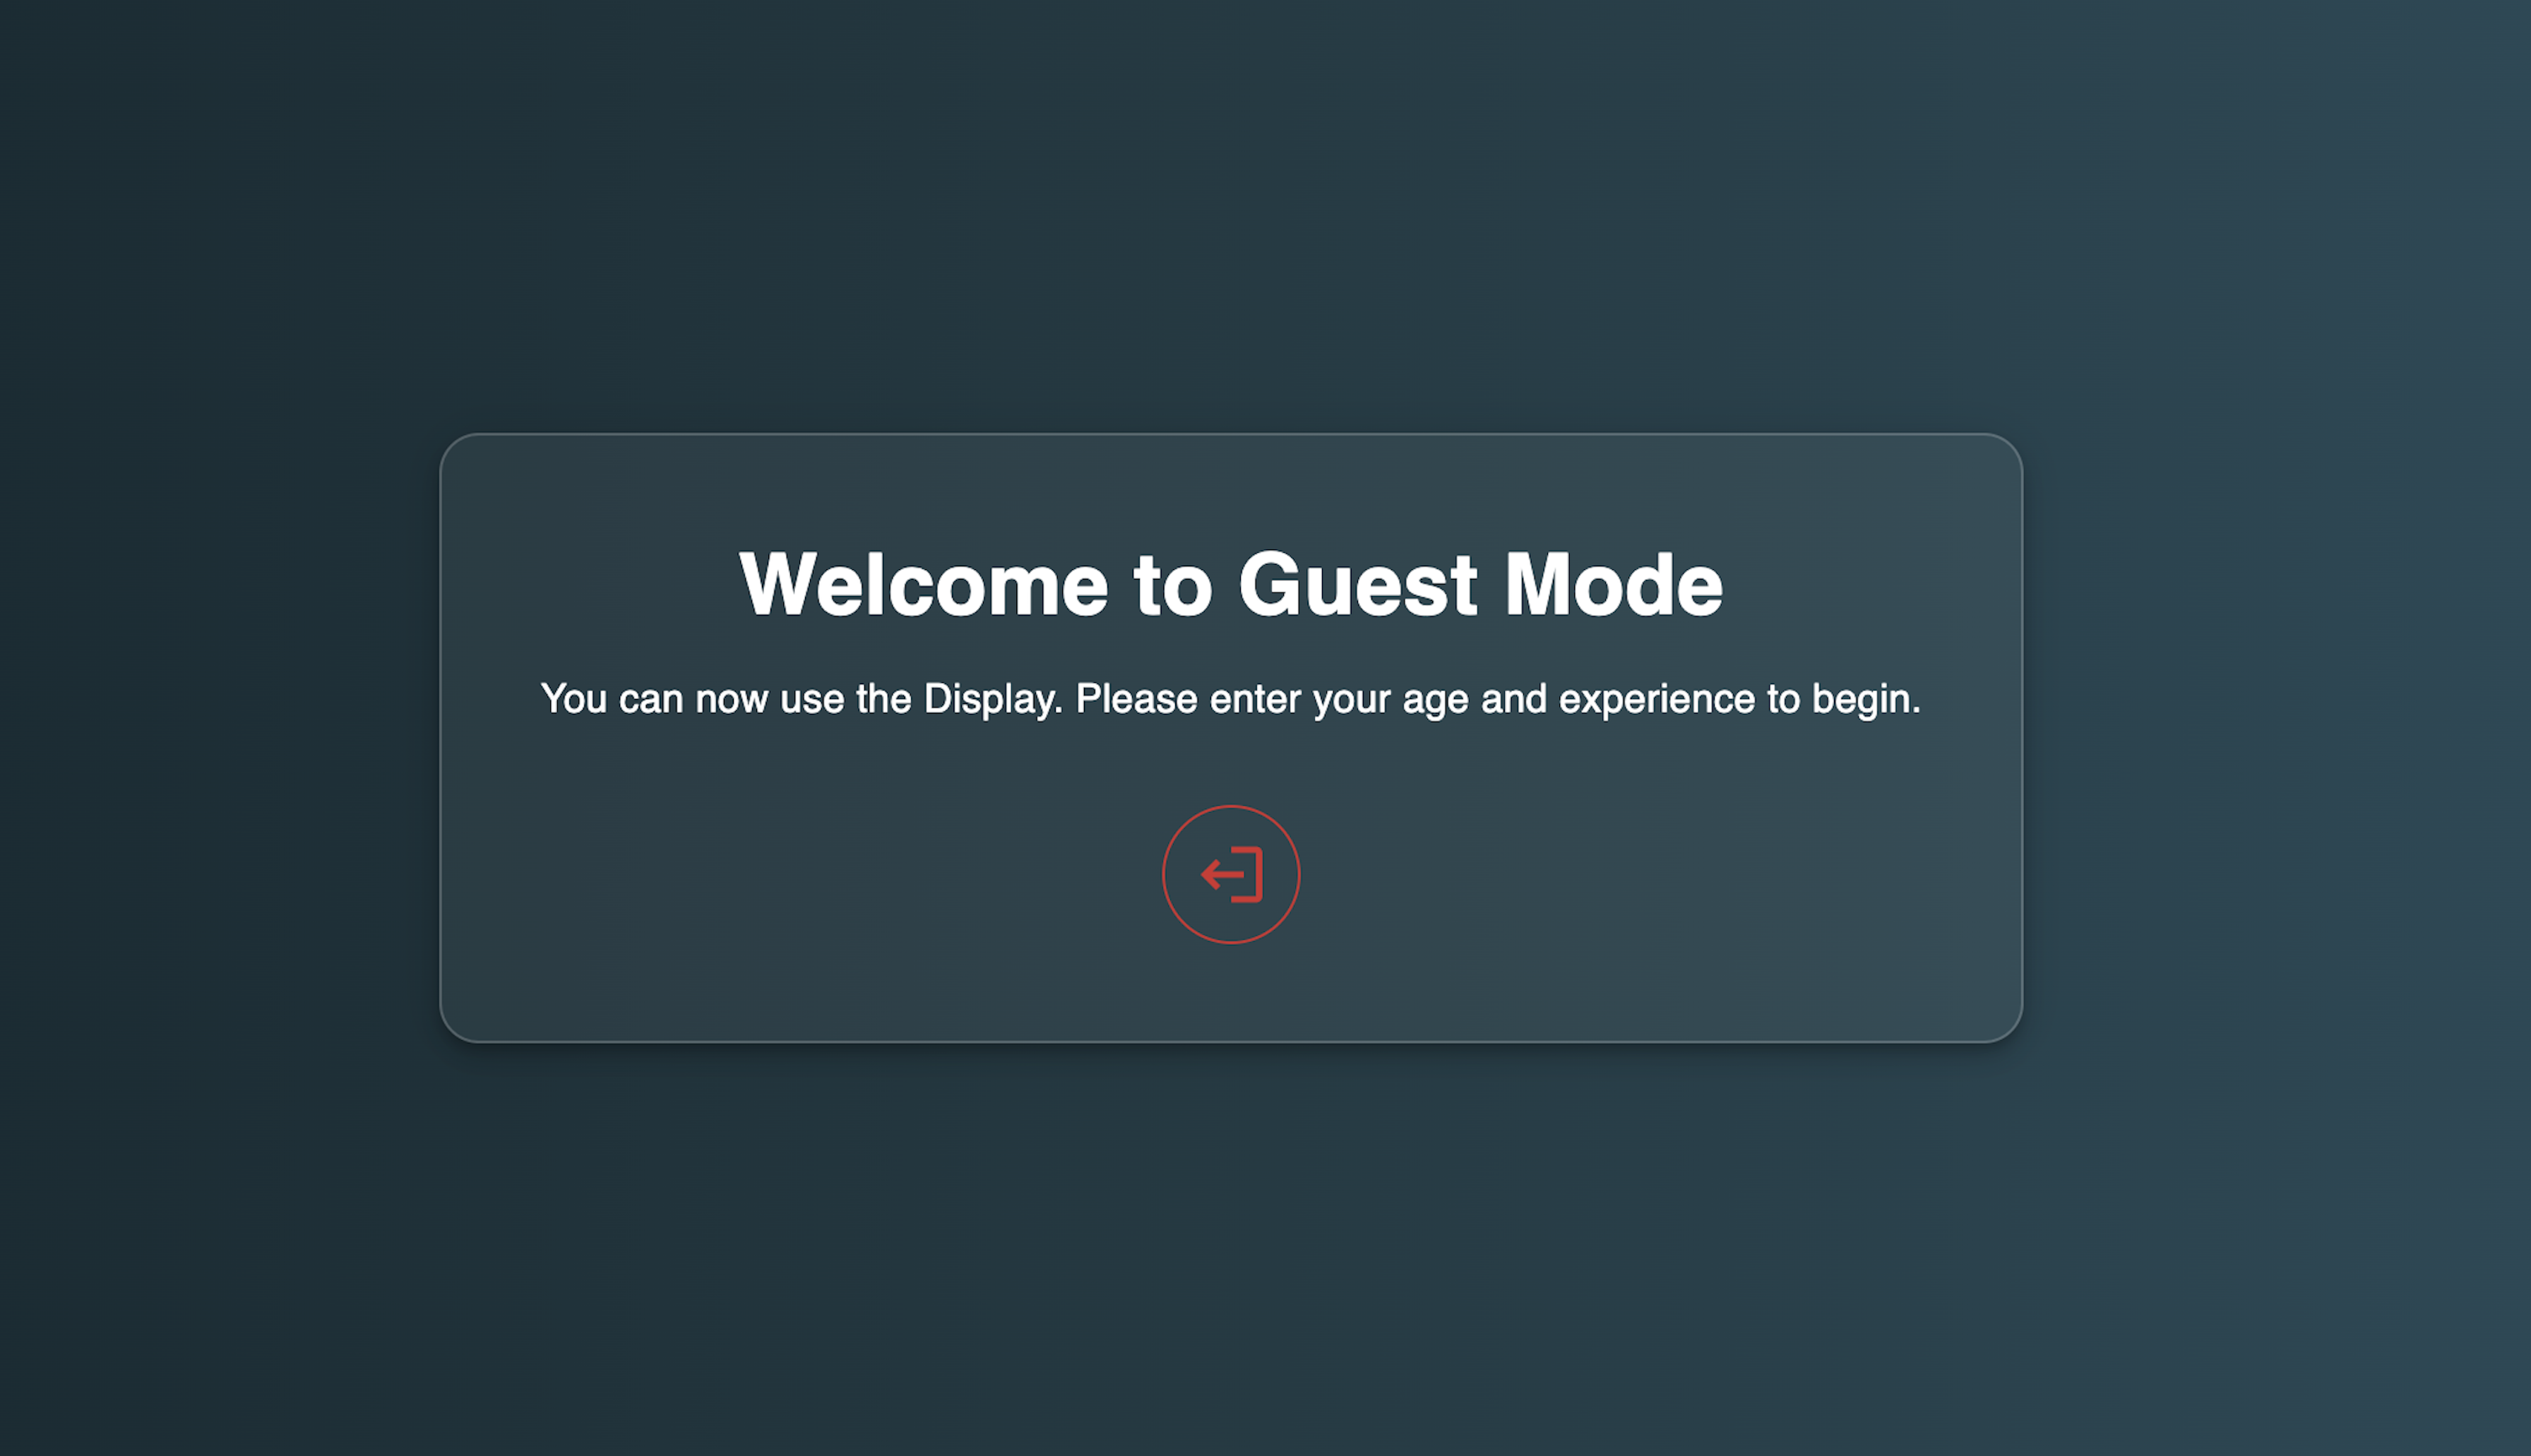
\includegraphics[width=0.6\textwidth]{images/WelcomeScreen.png}
    \caption{Connected as Guest-User example}
\end{figure}
When the user scans the QR code with their device, a screen will appear allowing them to leave the 
session remotely without needing to interact directly with the public display. 
If the user chooses the private mode, a \textbf{session token} linked to the user's device is stored on server side, preventing other 
user's from interfering with the same session.

\begin{figure}[H]
    \centering
    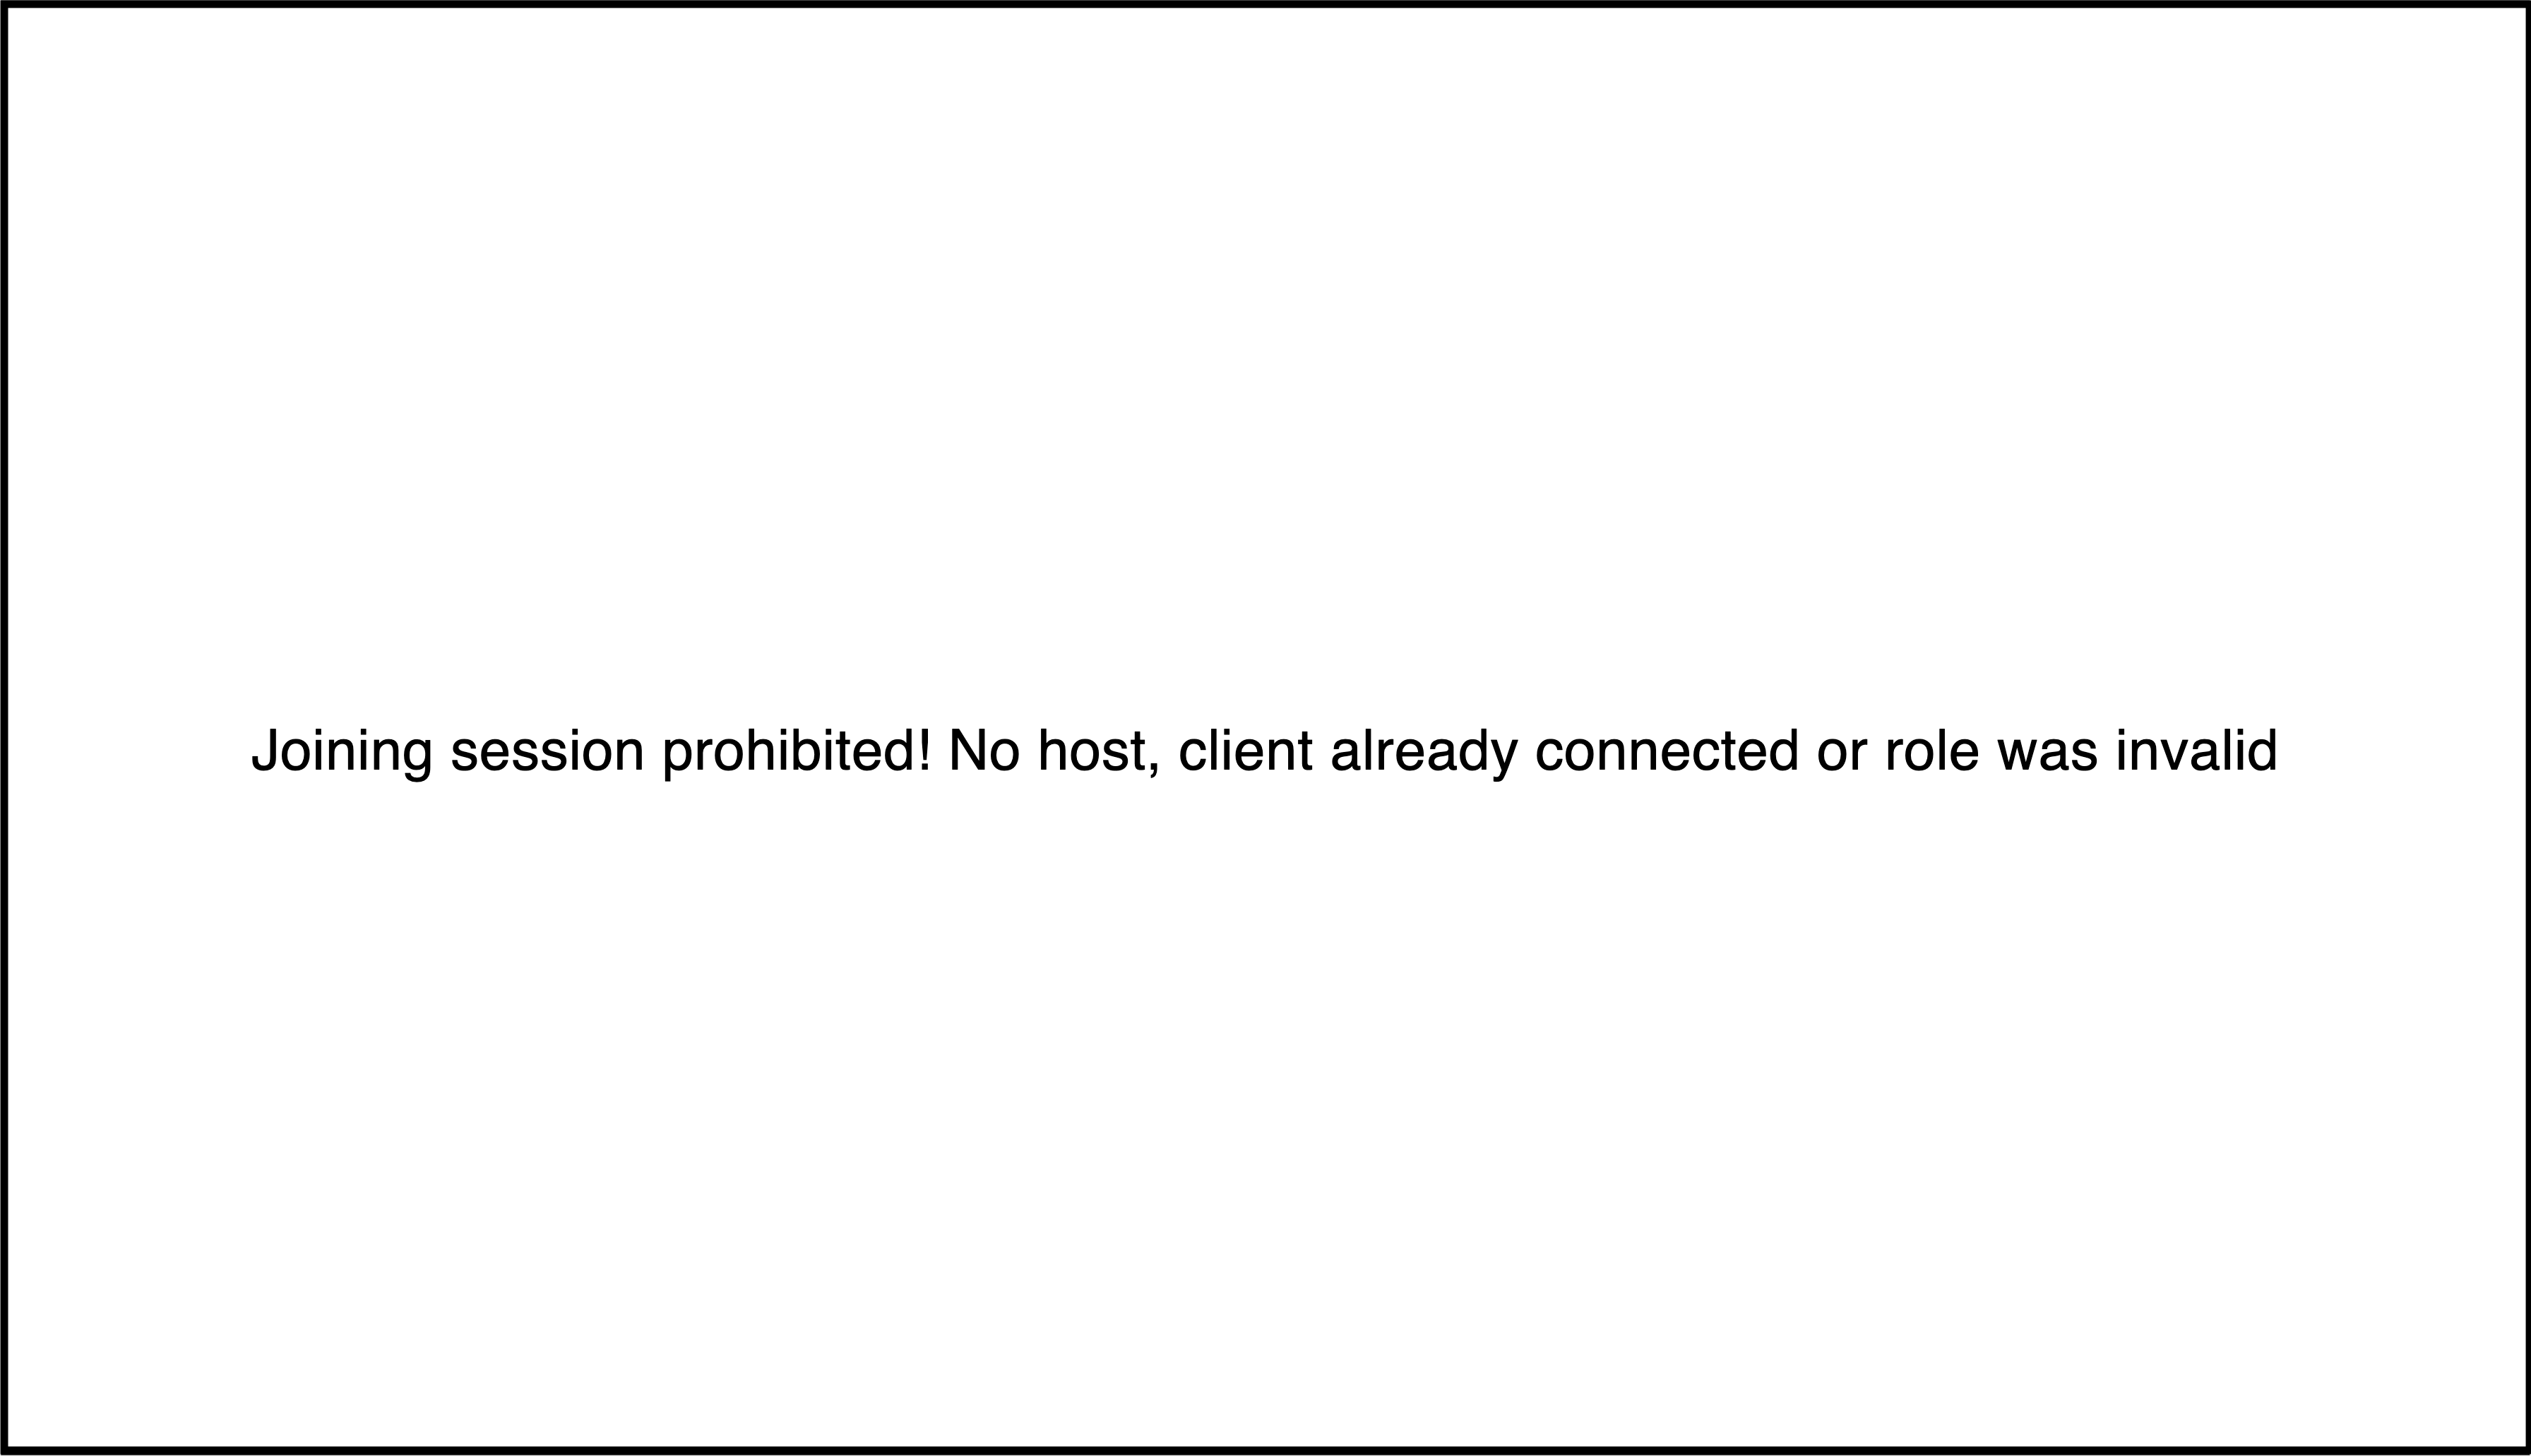
\includegraphics[width=0.6\textwidth]{images/WelcomeScreenInvalid.png}
    \caption{Forbidden connection example}
\end{figure}
If a user is already connected to the server, any subsequent user scanning the QR code will see 
a different screen on their device, informing them, that the \textbf{session is currently occupied}.